\subsection{Probabilistic Payment Channels}
\label{sec:incentives:probabilistic}

Payment channels give two nodes, $A$ and $B$, the opportunity to lock funds on-chain and later on handle who of them possesses which fraction. At each moment, it holds that

$$ balance(A) + balance(B) = const. $$

The state becomes final once one of the nodes submits the most recent state to the smart contract. Therefore it requires a proof by the counterparty that the proclaimed state is in their interest, which is given by a digital signature and named \textit{update transaction}. Hence an update transaction that transfers $x > 0$ digital assets from $A$ to $B$ is approved by,

$$ update_i = Sig_A (balance(A) - x \ || \ balance(B) + x) $$

By doing so, payments can only in one direction, turning the payment channel into a unidirectional payment channel. This is possible because digital assets will only be transferred from $A$ to $B$ and thus $B$ will always pick in its own the interest the most recent update transaction since $balance(B)$ is strictly increasing.

If the channel allowed asset transfers in the opposite direction, namely from $B$ to $A$ the update transactions need to include a versioning element that prevents any of the parties from rollback to the most beneficial state since the smart contract is unable to determine the most recent transaction otherwise. Hence,

$$ update_i = Sig_A (i \ || \ balance(A) - x \ || \ balance(B) + x) $$

In addition, this requires certain timeframes in which the counterparty is given the opportunity to present their most recent update transaction. This is necessary because none of the nodes can prove that there does \textit{not} exist a more recent update transaction. Once the timeout ends, and none of the parties have submitted any more recent update transaction, the last submitted state becomes final.

\begin{figure}[H]
    \centering
    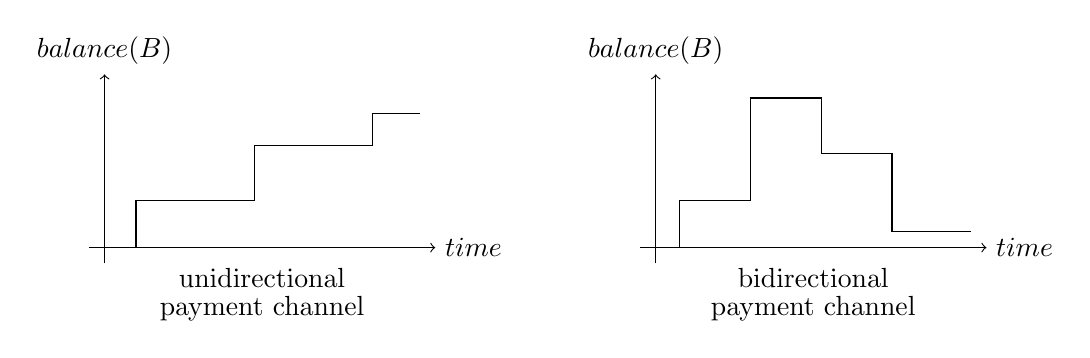
\begin{tikzpicture}[domain=0:2]
        \def\padding{0.1}
        \def\plotHeight{2}
        \def\plotWidth{4}
        \def\plotOffset{7}
        \def\textOffset{0.6}
        \foreach \i in {0,1} {
                \begin{scope}[shift={(\i*\plotOffset,0)}]
                    \draw[->] (-2*\padding,0) -- (\plotWidth+2*\padding,0) node[right] {$time$};
                    \draw[->] (0,-2*\padding) -- (0,\plotHeight+2*\padding) node[above] {$balance(B)$};

                    \ifnum\i=0
                        \path (0,-\textOffset) -- (\plotWidth,-\textOffset) node[midway] {\shortstack{unidirectional\\payment channel}};
                        \draw (0.4,0) -- (0.4,0.6) -- (1.4,0.6) -- (1.9,0.6) -- (1.9,1.3) -- (2.6,1.3) -- (3.4,1.3) -- (3.4,1.7) -- (4.0,1.7);
                    \else
                        \path (0,-\textOffset) -- (\plotWidth,-\textOffset) node[midway] {\shortstack{bidirectional\\payment channel}};

                        \draw (0.3,0) -- (0.3,0.6) -- (1.2,0.6) -- (1.2,1.9) -- (2.1,1.9) -- (2.1,1.2) -- (3.0,1.2) -- (3.0,0.2) -- (4.0,0.2);
                    \fi
                \end{scope}
            }
    \end{tikzpicture}
    \label{fig:channels}
    \caption{Node $A$ and $B$ have a payment channel. Whilst in case of unidirectional payment channels, $balance(B)$ is strictly increasing, the derivative of $balance(B)$ \textit{can} change sign if the channel is bidirectional.}
\end{figure}

Within the HOPR protocol, payment channels are implemented as unidirectional channels, hence there \textit{can} be one from $A \rightarrow B$ and another one from $B \rightarrow A$. Whenever, an update transaction is submitted to the blockchain, the assets get transferred to the channel in the opposite direction, or directly to the counterparty if there is no such channel. This obviously controverses the original purpose of payment channels, which is \textit{aggregation} of asset transfers.

When talking about unidirectional payment channels, aggregation means that $value(update_i) = value(update_{i-1}) + \Delta x$, hence $update_i$ makes $update_{i-1}$ obsolete as it already includes the additional assets $\Delta x$. So, if a node manages to receive $update_i$ before $update_{i-1}$, there is no need to provide the services the which were supposed to be compensated by $update_{i-1}$.

This is problematic for HOPR because it uses \nameref{sec:incentives:proofofrelay} to unlock payment made from one node to the other and the state of a payment channel between nodes $n_{i-1}$ and $n_i$ therefore relies on third-party actions, namely by $n_{i+1}$ and $n_{i+1}'$. Both of them acknowledge the reception of the packet and the correct transformation done by node $n_i$. Using update transactions arises the question which update transaction node $n_{i+1}$ and node $n_{i+1}'$ should sign because they cannot know which acknowledgement reaches $n_i$ first. Hence, the incentives for packet need to be done independently and thus should not rely on update transactions.

\begin{figure}[H]
    \centering
    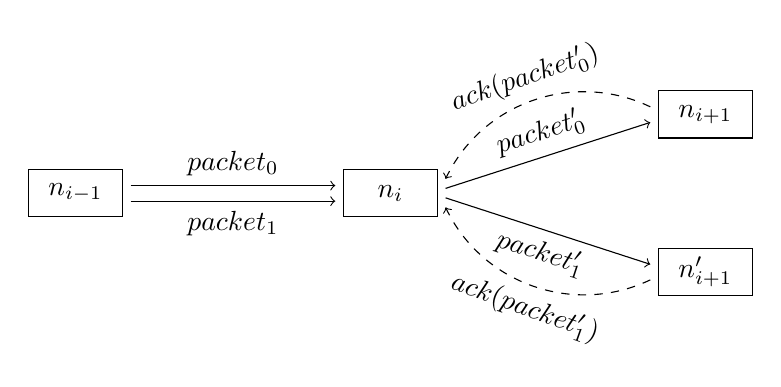
\begin{tikzpicture}
        \def\nodeOffset{4}
        \def\nodeYOffset{1}
        \def\nodeWidth{1.2}
        \def\nodeHeight{0.6}
        \def\padding{0.1}

        \foreach \xOffset\yOffset\name in{-\nodeOffset/0/$n_{i-1}$,0/0/$n_i$,\nodeOffset/\nodeYOffset/$n_{i+1}$,\nodeOffset/-\nodeYOffset/$n_{i+1}'$} {
                \draw[shift={(\xOffset,\yOffset)}] (0,0) rectangle (\nodeWidth,\nodeHeight) node[midway] {\name};
            }

        % Packets
        \draw[->,shift={(0,0.66*\nodeHeight)}] (-\nodeOffset+\nodeWidth+\padding,0) -- (-\padding,0) node[midway,above] {$packet_0$};
        \draw[->,shift={(0,0.33*\nodeHeight)}] (-\nodeOffset+\nodeWidth+\padding,0) -- (-\padding,0) node[midway,below] {$packet_1$};

        % Forwarded packets
        \draw[->] (\nodeWidth+\padding,0.6*\nodeHeight) -- (\nodeOffset-\padding,\nodeYOffset+0.33*\nodeHeight) node[midway,sloped,above] {$packet_0'$};
        \draw[->] (\nodeWidth+\padding,0.4*\nodeHeight) -- (\nodeOffset-\padding,-\nodeYOffset+0.66*\nodeHeight) node[midway,sloped,below] {$packet_1'$};

        % Acknowledgements
        \draw[->,dashed] (\nodeOffset-\padding,\nodeYOffset+0.66*\nodeHeight) to [bend right=45] node[above,sloped] {$ack(packet_0')$} (\nodeWidth+\padding,0.8*\nodeHeight);
        \draw[->,dashed] (\nodeOffset-\padding,-\nodeYOffset+0.33*\nodeHeight) to [bend left=45] node[below,sloped] {$ack(packet_1')$} (\nodeWidth+\padding,0.2*\nodeHeight);
    \end{tikzpicture}
    \caption{Node $n_{i-1}$ send packet $packet_0$, $packet_1$ to node $n_i$ which forwards them to node $n_{i+1}$ and node $n_{i+1}'$. Both nodes acknowledge the validity of $packet_0'$ and $packet_1'$ to node $n_i$.}
    \label{fig:sharedpaymentchannel}
\end{figure}

\paragraph{Probabilistic payments}
\label{sec:incentives:probabilistic:probabilistic}

Incentives relate to packets which are assumed to be sent very often in the HOPR network. Nodes can therefore expect that they will shortly receive another micropayment from the same node. It is thus not necessary to claim the incentive for each packet individually. This is why nodes issue each other probabilistic \lcnameref{sec:tickets} that have the same asymptotic payout but do neither require in-order processing nor require an on-chain operation for every incentive. Hence when picking the same relay fee, it holds that

$$ \forall i \ \forall j \ : \ value(ticket_i) = value(ticket_j) $$

Moreover, the nodes estimate the usage of the link to the nodes with whom they have engaged in a payment channel and pick a ticket winning probability that leads to a continous payout. Connections with higher througput can use lower probabilities whilst those with fewer traffic are supposed to use winning probabilities closer to 1.

Probabilistic payments rely on the necessity for the ticket issuer to not know whether a ticket that is issued will turn into an asset transfer or not. Hence, the ticket redemption must rely on some entropy provided by the ticket redeemer and need to be kept secret until the ticket is redeemed. This is necessary, because by knowing which ticket is going to become a winner, the ticket issuer would solely issue losing tickets and thereby withhold the incentives for the next downstream node.

Analogously, the ticket receiver should not know whether a ticket will be a win before being able to reconstruct the response to the challenge stated in the ticket. If not, the ticket receiver would just process those packet that come with a winning ticket and drop all other packets.

A ticket is a winner if

$$ keccak256 ( ticketHash \ || \ porSecret \ || \ opening) < ticket.invWinProb $$

where $ticketHash$ is the hash of the received ticket, see section \ref{sec:tickets:redemption}, and thus known by both ticket issuer and recipient whereas $porSecret$ is known by the ticket issuer and can be reconstructed as part of the $\nameref{sec:incentives:proofofrelay}$ scheme by the ticket recipient once it receives the acknowledgement for the forwarded ticket. On the other hand, $opening$ refers to the value that opens the most recent commitment that is stored on-chain, see section \ref{sec:incentives:commitment}. The on-chain commitment is chosen by the ticket recipient and due to the hiding property of the utilized commitment scheme, the opening values are solely known by the ticket recipient.